\setstretch{2}
\section{Chapter Summary}
\section{FAD as a marker for metabolic health in the retina}\label{sec:FADderivation}
Mapping the concentration of FAD would enable the diagnosis of retinal disease before physical damage to eyesight develops, at the stage of metabolic dysfunction. FAD is a flavoprotein produced in the body as a by-product of oxygen metabolisation from aerobic respiration (\cref{eq:resp})~\cite{berg2007biochemistry} to create ATP - the bodies source of energy. In the formation of retinal disease, the retina would exhibit abnormal metabolic activity - ATP usage - and would present in the retina as areas with abnormal FAD distribution.
\begin{equation}\label{eq:resp}
    \ce{C6H12O6 + 6O2 -> 6CO2 + 6H2O + ATP}
\end{equation}
While the magnitude of the changes in retinal FAD distribution associated with retinal disease is not know attempts can be made to detect the presence of FAD and assess it feasibility as a diagnostic tool. Changes in FAD concentration can be anaesthetised in animal models by artificially restricting systemic oxygen consumption producing a detectable change in the SFLIM measurements. In normoxic conditions, (\qty{21}{\percent}\ce{FiO2}, oxygen metabolism is typical however in hypoxic conditions (\qty{15}{\percent}\ce{FiO2}) the retina is starved of oxygen thus lowering the detectable concentration of FAD. After death when all metabolic processes have cease the concentration of FAD should tend to zero - in rat cortexes this has been reported as the FAD leaking out of arteries forming `halos'~\cite{martinez2017understanding}.
In this chapter, the SFLIO device (described in~\cref{chap:fliodevice}) was used to record \textit{in-vivo} SFLIM images of the retinas of anaesthetised rats under normoxic, hypoxic, and post-mortem conditions where the concentration of retinal FAD is recovered using the SFLIM unmixing algorithm (described in \cref{chap:tensSFLIM}). Successful detection of FAD is then signified by the changes in the recovered retinal FAD concentration being compatible with what is expected with aerobic respiration. Finally, from this a feasibility of quantifying retinal FAD in human retinas can explored.
\subsection{Estimating The Change in Retinal FAD Concentration at Hypoxia}
The expected variation in FAD concentration as a response to changing oxygenation can be modelled by estimating the rate of FAD production due to oxygen metabolisation in the retina at both normoxia, and hypoxia.
The rate at which oxygen is metabolised $Q_{\ce{O2}}$ is calculated using~\cref{eq:O2rate} from the average rate of blood flow through the ophthalmic artery, $Q_{ret}$, and the relative change in saturation of blood entering, ${S\ce{O2}}_{in}$, and exiting, ${S\ce{O2}}_{out}$, it.
\begin{equation}\label{eq:O2rate}
    Q_{\ce{O2}} = Q_{ret}({S\ce{O2}}_{in}-{S\ce{O2}}_{out})H
\end{equation}
The rate of blood flow through the ophthalmic artery was taken as $Q_{ret} = \qty{41.35}{\micro\litre\per\minute}$ by averaging two reported measurements in literature~\cite{dai2013absolute,riva1985blood}. The oxygen saturation - the ratio of oxygenation to deoxygenated haemoglobin in the blood - has been reported as \qty{92.20}{\percent} and \qty{55.60}{\percent} for blood entering and exiting the ophthalmic artery~\cite{dunn2016physiology}. Using~\cref{eq:O2rate} the rate of oxygen metabolisation was estimated to be $Q_{\ce{O2}}=\SI{3.155}{\micro\litre\per\minute}$ where $H=\num{0.2085}$ is H{\"u}ffners constant which is the volumetric ratio of oxygen to haemoglobin in the blood~\cite{dunn2016physiology}. 
The rate of FAD production, $Q_{FAD}$, can then be determined by considering that for every metabolised \ce{O2} molecule $k_{FAD} = 3$ molecules of FAD are produced with an efficiency of $\eta_{FAD} = \qty{1.3}{\percent}$~\cite{berg2007biochemistry,ames1992energy}.
\begin{equation}
    Q_{FAD} = Q_{\ce{O2}}k_{FAD}\eta_{FAD}
\end{equation}
This yields a production rate of $Q_{FAD} = \qty{0.123}{\micro\litre\per\min}$ which is then be converted to a steady state volume of FAD by assuming that all FAD in the retina is produced in the time taken for blood to flow through the retina and any FAD that is consumed is replaced upon the next circulation period of blood. With a blood flow period of $\delta T = \qty{4.7}{\second}\equiv \qty{0.078}{\minute}$ measured as the time interval between blood entering and exiting the ophthalmic artery~\cite{khoobehi1990measurement}.
\begin{equation}
    V_{FAD} = Q_{FAD}\delta T
\end{equation}
With this calculated volume of retinal FAD,$V_{FAD} = \qty{9.639}{\nano\litre}$, corresponds to $N_{FAD} = \qty{12.27}{\nano\mole}$ using~\cref{eq:nummoles} with a $gfm_{FAD} = \qty{785.56}{\gram\per\mole}$, a density equal to that of water of $\rho_{FAD} = \qty{1}{\gram\per\milli\litre}$, and $N_{A} = \qty{6.022e23}{\per\mole}$.
\begin{equation}\label{eq:nummoles}
    N_{FAD} = V_{FAD}\rho_{FAD}gfm_{FAD}
\end{equation}
Finally, the result of~\cref{eq:nummoles} is expressed as a concentration by approximating the retina as a cuboid with thickness of \qty{344}{\um} and surface area of \qty{1361}{\milli\metre\squared} to estimate its volume~\cite{nagra2017determination,myers2015retinal}.
\begin{equation}\label{eq:FADconc}
    C_{FAD} = \frac{N_{FAD}}{V_{ret}} = \SI{26.9921}{\micro\mole\per\litre}
\end{equation}
While this analysis does represent a simplified interpretation of the biological functions in the retina it is commensurate with reported measurements of flavoproteins in rabbit eye's. In~\citeauthor{batey1991analysis}\cite{batey1991analysis}, the concentration is defined as \qty{39.3}{\pico\mole\per\milli\gram} by weight of the retina which is within \qty{10}{\percent} of the estimation above when converted to equivalent units - $C_{FAD} = \qty{37.64}{\pico\mole\per\milli\gram}$ obtained using the result of \cref{eq:nummoles} and taking the mass of the retina as \qty{326}{\milli\gram}~\cite{batey1991analysis,feke1989blood}.
\\
The volume of FAD in the retina at hypoxia can then be estimated by assuming that the drop in maximal oxygen consumption, ${\dot{V}\ce{O2}}_{max}$, due to hypoxia will induce a decrease in the volume of retinal FAD of an equal order. This rate of maximal oxygen consumption was measured of sedentary and endurance trained subjects as reported in~\citeauthor{ferretti1997decrease}\cite{ferretti1997decrease} and shown in \cref{tab:VO2max}. 

\begin{table}[htb]
    \centering
    \begin{tabular}{|c|c|c|}
    \hline
    \ce{FiO2} & \multicolumn{2}{c|}{${\dot{V}\ce{O2}}_{max}$ (\si{\litre\per\minute})}\\
    \cline{2-3}
    & Sedentary & Athletic\\
    \hline
    \qty{21}{\percent} & \num{3.13} & \num{4.11}\\
    \qty{13}{\percent} & \num{2.27} & \num{2.92}\\
    \hline
    \end{tabular}
    \caption{In \citeauthor{ferretti1997decrease}\cite{ferretti1997decrease}, the maximal rate of oxygen consumption was measured of sedantary subjects and subject with a background in endurance sports for a range of inspired oxygen concentrations (\ce{FiO2}). Reproduced from Table. 1 of \citeauthor{ferretti1997decrease}\cite{ferretti1997decrease}.}
    \label{tab:VO2max}
\end{table}
The ratio between the hypoxic and normoxic measurements of ${\dot{V}\ce{O2}}_{max}$ are then $\Gamma = \num{0.725}$, and $\Gamma = \num{0.710}$ for sedentary and athletic subjects, receptively. Taking the case of a sedentary subject the volume of FAD at hypoxia is $V_{FAD,hypoxia} = \Gamma V_{FAD, normoxia} = \qty{6.839}{\micro\litre}$ and the concentration of FAD at hypoxia is estimated as $C_{FAD,hypoxia} = \Gamma C_{FAD, normoxia} = \qty{19.164}{\micro\mole\per\litre}$. \\
In the SFLIM measurements of anaesthetised, hypoxic, rats, the relative mean concentration of FAD it would be expected to be on-the-order of \qty{30}{\percent} lower than the recorded FAD concentration measured of normoxic rats. Although measurements of the concentration of retinal FAD, nor measurements of oxygen saturation in the for hypoxia and normoxic retinas have not been reported for rats this analysis is still useful for confirming that FAD concentration would be expected to decrease under acute hypoxia (\ce{FiO2}) \qty{15}{\percent}. In humans, the decrease of oxygen saturation in the retina, due to acute hypoxia, was reported by \citeauthor{choudhary2013assessment}\cite{choudhary2013assessment}, as \qty{8.2}{\percent} and \qty{8.3}{\percent} for arterial and venous blood, respectively. From this, it could be concluded that a decrease in retinal FAD of $\approx\qty{8}{\percent}$ would be expected due to acute hypoxia. However, as a result of acute hypoxia in humans, the retinal blood vessels dilate by a factor of between \qtyrange{3.5}{21}{\percent}\cite{choudhary2013assessment,frayser1971response} and according to Poiseuille's Law (\cref{eq:poislaw})~\cite{westerhof2019law}.
\begin{equation}\label{eq:poislaw}
    \Delta P \propto  \frac{Q}{r^{4}}
\end{equation}
This causes a fourth-power increase in the rate of blood flow, $Q$, assuming equal blood pressure, $\Delta P$, for an increasing radius of blood vessel, $r$. For the above dilation factors this would represent an increase in venous blood flow of \qtyrange{16}{114}{\percent}. The affect of increased venous blood flow could imply the concentration of retinal FAD would paradoxically increase as a result of acute hypoxia. This underpins the need for quantitative measurements of retinal fluorophores such as those carried out and presented in this chapter.
\FloatBarrier
\section{\textit{In-Vivo} SFLIM Measurements of Anaesthetised Rats}
\subsection{Experimental Protocol}
The reported imaging experiments were carried out in the labs of Prof. Kenneth J. Smith (Institute of Neuroinflammation, UCL) where Helen Yang (Institute of Neuroinflammation, UCL) prepared the rats for imaging, administered isoflurane to anaesthetise them, and monitored health throughout the imaging session. An external nitrogen supply was mixed with room-air and fed into a fitted nose-cone to control the fraction of inspired oxygen between. Albino rats were chosen for their lack of melanin in the eye which reduces the loss of emitted retinal autofluorescence to absorption and maximising SNR in detected fluorescence. As shown in~\cref{fig:ratsetup}, the rat is secured to the imaging platform and the pupil is dilated using Tropicamide drops to increase pupil diameter (\qtyrange{1.20}{4.35}{\mm}~\cite{himmel2019pupillary}) - maximising the number of detected photons. The eye lids are fixed open with stitches and contact lens is fitted to index-match the rats eye lens. Viscotears gel is applied around the cornea to prevent the eye becoming dry and irritated - inducing additional eye movement and motion requiring correction. To accommodate the rats smaller eyeball diameter, of \SI{6.3}{\mm}~\cite{pazos2015rat}, a field-lens ($\varphi = 2''$, $f = \SI{85}{\mm}$) is fitted to the objective lens of the fundus camera. This additional lens did induce reflections from the illumination source off the front surface of the objective lens and rear surface of the field lens degrading some of the brightfield images with glare (\cref{fig:Ratscmosimages}a) with the penalty of reducing the effectiveness of the motion detection process. This glare was observed to be independent of the motion of the retina which would cause errors in the detected motion in the phase-cross correlation process. By multiplying the images by a mask that is zero in the glare-affected areas and unity elsewhere, the effects of glare was satisfactorily mitigated.  Alternatively, the glare could be removed using an image recorded of a non-reflective scene containing only the glare ($I_{dark}$) and linearly subtracting it from an recorded image ($I_{raw}$) to produce a glare-free image: $I = \alpha I_{raw} - I_{dark}$. 


\begin{figure}
    \centering
    \begin{annotatedFigure}{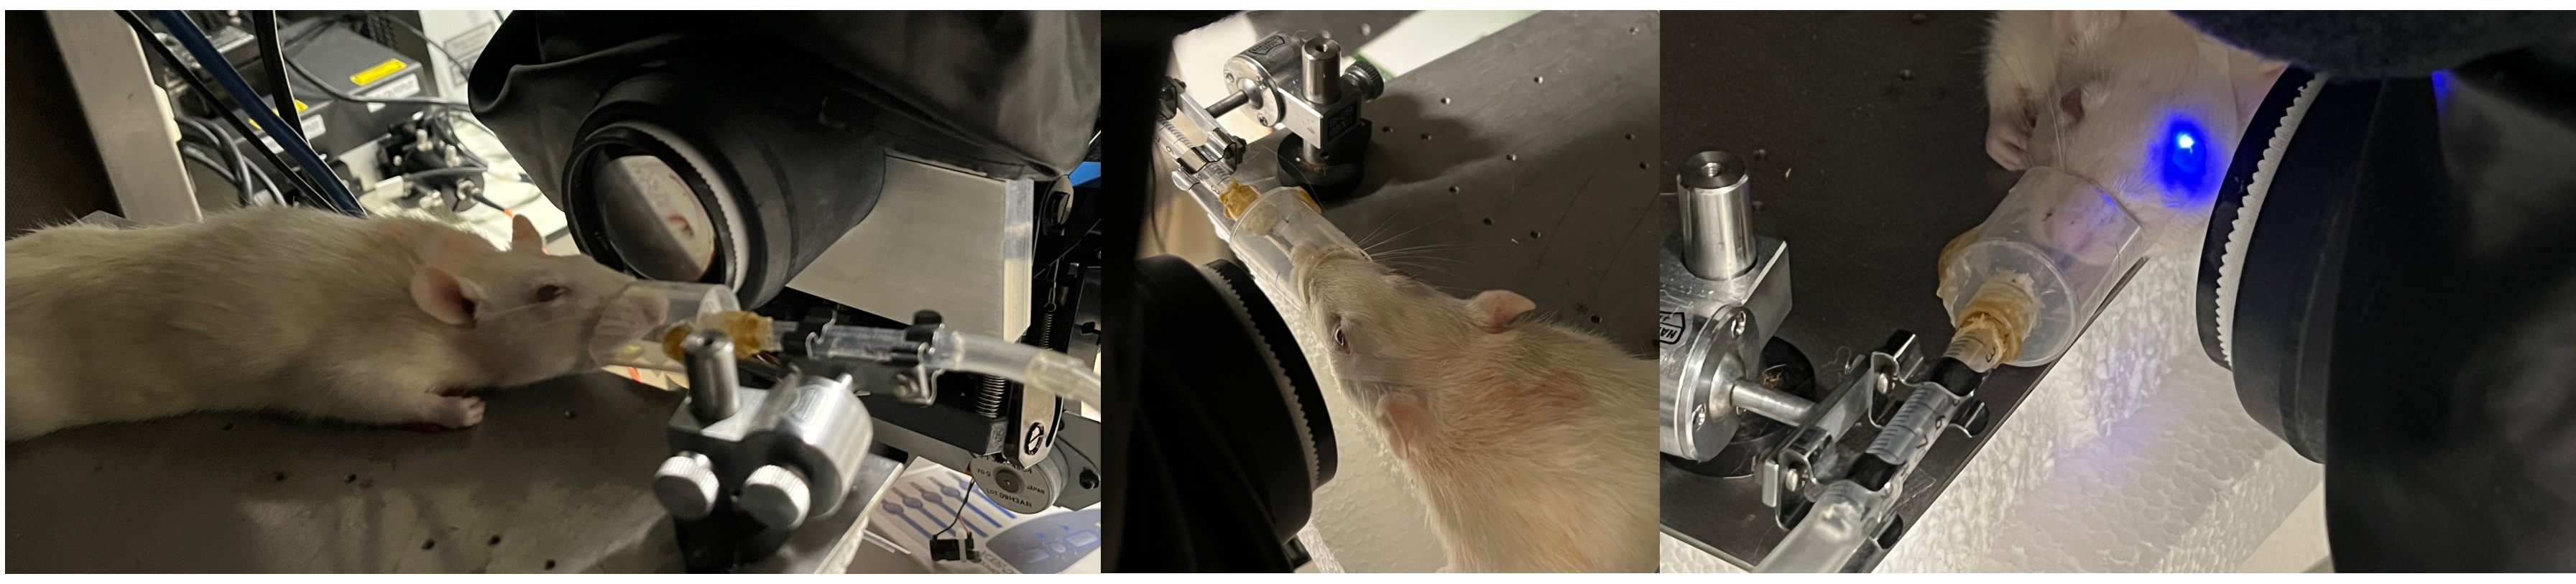
\includegraphics[width = \textwidth]{figures/ratUCL/RatSetupFigure.pdf}}
        \annotatedFigureText{0.015,0.83}{white}{0.3}{a)}
        \annotatedFigureText{0.435,0.83}{white}{0.3}{b)}
        \annotatedFigureText{0.66,0.83}{white}{0.3}{c)}
    \end{annotatedFigure}
    
    \caption{a) and b) The anaesthetised rat is positioned on the imaging platform perpendicular to the SFLIO system to have the rat's retina parallel with the image plane. The fundus camera is moved axially such that the illumination forms a focussed spot on the cornea - evenly illuminating the retina (c).}
    \label{fig:ratsetup}
\end{figure}
Two rats were imaged over three days. For each acquisition brightfield images are recorded continuously (\SI{50}{\ms} exposure at \SI{10}{\Hz}) in tandem with the FLIMera operating in raw mode over a two minute acquisition period for all 5 spectral filters. Due to the large file size generated from the FLIMera RAW acquisition around \SI{10}{\minute} is required the build and save the \SI{50}{\giga\byte} stream of photon counts for each spectral channel. This SFLIM acquisition is carried out while the rats are cycled from normoxia to hypoxia (\SI{15}{\percent}\ce{FiO2}) and then back to normoxia again with an $\approx 5$~minute interval between each acquisition. These intervals between spectral filters and oxygenation states minimises any photobleaching and should ensure that metabolic processes and FAD concentration re-stabilise although long periods of hypoxia can cause the rat to die due to oxidative stress. SFLIM images were recorded for the first rat on the second day. As before (\cref{fig:flimerascmossync}), the two detectors are synchronised in time by initially having the laser shutter closed at the start of the acquisition and then opening it after a short period of time and detecting the Heaviside-like change in photon flux. Due to the anaesthetic the nervous response in the rats is suppressed which eliminates any visible saccades in the image sequence. The motion correction algorithm developed in \cref{chap:motionreg} is still utilised to ensure any small movements of the rat over the hour long imaging sessions does not cause misalignment between spectral filters. However due to the no pixel super-sampling was performed (\cref{fig:FLIMerareg}c).

\begin{figure}
    \centering
    \begin{annotatedFigure}{\includegraphics[width = \textwidth]{figures/ratUCL/RatsCMOSfigure.pdf}}
        \annotatedFigureText{0.025,0.91}{white}{0.3}{a)}
        \annotatedFigureText{0.35,0.91}{white}{0.3}{b)}
        \annotatedFigureText{0.68,0.91}{white}{0.3}{c)}
        \annotatedFigureText{0.19,0.425}{white}{0.3}{d)}
        \annotatedFigureText{0.52,0.425}{white}{0.3}{e)}
    \end{annotatedFigure}
    \caption{a - c) Shows example brightfield images recorded of each of the 3 rats imaged. Each frame is recorded over an integration time of \SI{30}{\ms} at a rate of \SI{10}{\Hz} where a small amount of glare is present in the highlighted region of a). In d) and e) a fluorescence intensity image was recorded using a \SI{500}{\nm} long-pass filter over integration times of \SI{1}{\second} and \SI{5}{\second} respectively.}
    \label{fig:Ratscmosimages}
\end{figure}
\FloatBarrier
\subsection{Detected Translational Motion in Rat Retinas}
As discussed in \cref{chap:motionreg}, compensation of retinal motion is required for producing a high-contrast image where the vasculature is sharply defined. This would enable any variation in the distribution of FAD in the retina to be resolved with high confidence. Retinal motion is detected from image sequences by computing the phase-cross correlation between a reference image and each successive frame in the sequence - where this reference image is the first fully illuminated frame in the sequence after the laser shutter has been opened. This process was carried out for each spectral channel in the SFLIM acquisition and it was found a simple model of translational motion was sufficient for producing a brightfield image free of motion artefacts (see figure). 

However, in one instance the rat exhibited laboured breathing causing motion that was not just horizontal and vertical translations (see the video sequence titled ``DGeddesPhD\_RatBreatingMotion.mp4''). The differences in image magnification or rotation were small enough in amplitude and frequency that motion can be adequately corrected and characterised using the previously described method in \cref{chap:motionreg}. 


\begin{figure}
    \centering
    \includegraphics[width = 0.9\linewidth]{figures/ratUCL/RatMotionFigure.pdf}
    \caption{Montage of brightfield image sequence recorded at normoxia after the rat had previously been acutely hypoxia (\SI{12}{\percent}\ce{FiO2}) for a period. Laboured breathing in the rat caused artefacts in the sequence as show above. This is better resolved by viewing the supplementary video ``DGeddesPhD\_RatBreatingMotion.mp4''. This motion is correctable using the existing motion correction algorithm discussed elsewhere \cref{fig:ratbreathcorrection}}
    \label{fig:ratbreathmotion}
\end{figure}

From \cref{fig:ratbreathcorrection}, the frequency of the breathing motion was estimated from the time between local minima in the detected translational shifts and was found to be \qtyrange{1}{1.2}{\hertz} corresponding to a heart rate of \numrange{60}{72} beats-per-minute. This motion also does not manifest as artefacts or reduced contrast in retinal vasculature within the image as can be seen in \cref{fig:ratbreathcorrection} where the an image formed from summing frames over the entire sequence with and without correcting for motion are indistinguishable.

\begin{figure}
    \centering
    \includegraphics[width=0.9\linewidth]{figures/ratUCL/RatBreathCorrection.pdf}
    \caption{The motion due to laboured breathing does not introduce artefacts in images formed from summing frames over the entire sequence before (left) and after (right) the motion is corrected. These two images are also broadly indistinguishable from a single elemental in the sequence (middle). The translational motion in the X (horizontal) and Y (vertical) directions is plotted (bottom) and shows the periodic nature of the breathing motion.}
    \label{fig:ratbreathcorrection}
\end{figure}
Importantly, the amplitude of the breathing motion is small enough that $\approx \num{10}$ pixels on the would manifest as $\approx \num{2}$ pixels on the FLIMera.
\FloatBarrier
\subsection{Addressing Lack of Spatial Variation in SPAD Images}
From these imaging experiments, whilst a brightfield image of the retina could be recorded  with sufficient contrast in the blood vessels - a image with clearly defined vessels could not be formed on the FLIMera. The exact cause of this is unknown but is worth exploring.
\begin{figure}
    \centering
    % \includegraphics[width=0.5\linewidth]{}
    \caption{C\textcolor{red}{To Do: Figure of a fluorescence intensity image recorded with the flimera of a rat}}
    \label{fig:ratflimcontrast}
\end{figure}
Since both detectors are focussed at infinity, when a brightfield or fluorescence image is formed on the sCMOS camera, a complimentary image should be formed on the FLIMera. Before the rats were imaged a sample of convallaria was mounted in the retinal plane of an artificial eye model and brightfield, and fluorescence intensity images were recorded with the sCMOS and FLIMera, respectively. The images were then registered as before in \cref{chap:motionreg} to obtain the affine transform between the detectors - this rules out poor focussing of the camera lenses as the culprit. 
The field lens used to accommodate the smaller, \qtyrange{2}{4}{\mm} diameter pupil of the rat could have caused poor focus in the SPAD image but this is also unlikely since a clear image could be resolved on the sCMOS detector. With the benefit of hindsight, a more rigorous method of evaluating this would be to use a divergent laser source to fill the aperture of the objective lens on the SFLIO device, with the field lens fitted, to ensure that a collimated beam is produced out of lens $f_{1}$. The detectors would then be focused when a focussed spot is produced on the detector - with laser power attenuated so as not to over expose or damage either detector.
Other sources of this lack of spatial variation were also hypothesised but were not experimentally investigated: autofluorescence due to the viscotears used to prevent the cornea drying out; excitation light due to the glare sport bleeding through. The viscotears gel is uses the active ingredient of poly-acrylic acid to prevent drying of the cornea with the sweetener, sorbitol (a sugar alcohol), and sodium hydroxide as preservatives. From an analysis of the available literature: poly-acrylic acid \cite{xu2019autofluorescence} is not intrinsically fluorescent and only fluoresces when forming hydrogels; sorbitol only emits fluorescence in the near-infrared wavelengths $\lambda >\qty{800}{\nm}$~\cite{lee2019near} which would be blocked by the anti-reflection coatings on the lenses within the SFLIO device; and sodium hydroxide only weakly emits fluorescence between \qtyrange{300}{440}{\nm} when excited at \qty{240}{\nm} and, importantly, only at a hazardous molar concentration of \qty{3}{\mole\per\litre}~\cite{villa2019anomalous} that could not be present in the viscotears gel. Measuring the spectral-temporal fluorescence properties of the viscotears gel would have experimentally demonstrated this. However, this brief review of the literature shows that not the root cause of the inability to produce a focussed image on the FLIMera was not likely to be the viscotears gel.
Reflected excitation light from the field-lens - which produced the glare spot in the brightfield images - could have not been sufficiently blocked by the emission filters resulting in $\approx \qty{0.2}{\micro\watt}$ out of the $\approx \qty{2}{\milli\watt}$ excitation source being transmitted through a filter with optical density, $\text{OD} = 4$ which could be sufficiently intense to contaminate the image. Fluorescence intensity images of the rat retinas were also recorded of the rat retina using the sCMOS detector and a \qty{500}{\nm} long-pass filter with $\text{OD} = 4$ and retinal vasculature were well defined and resolvable (see \cref{fig:Ratscmosimages}d-e).
\\
Despite the lack of spatial variation in the SPAD images, the SFLIM unmixing algorithm can still be utilised to determined whether we can detect a change in retinal FAD as a response to acute-hypoxia by averaging over the entire retina. This is explored in proceeding sections.
\FloatBarrier
\section{Recovering FAD Concentration Using SFLIM Unmixing}
Although clear images of the retina could not be formed on the FLIMera, the concentration of retinal FAD can be estimated over the entire FOV using the previously developed SFLIM unmixing algorithms. The SFLIM unmixing method was applied to SFLIM data with and without the application of motion correction. The relative concentrations of retinal fluorophores for each pixel on the FLIMera and the mean concentration can be calculated after masking out malfunctioning pixels with the pixel mask discussed in \cref{sec:pixelmask}. The recovered fluorophore concentrations were then compared over the Normoxia, Hypoxia, Re-Normoxia, and in one case \textit{post-mortem} to establish if the detected changes fitted the predictions made in \cref{sec:FADderivation}. The statistical significance was calculated using a paired student t-test to establish whether a change in retinal fluorophore concentration was detected as a result of a change in the rats physiology (\textcolor{red}{theres probably a better term for this}) or just due to noise. Finally, Principle Components Analysis (PCA) to assess whether the detected changes are due to changes in the fluorescence emission spectra or the fluorescence lifetime.
\FloatBarrier
\subsection{Darkfield Correction}\label{subsec:darkfield}
In the first two of three imaging sessions the fluorescence decay was contaminated by a dark current which appeared as a Gaussian-like function superimposed onto the fluorescence decay (see \cref{fig:darkfieldGauss}). Darkfield FLIM measurements were recorded with the FLIMera covered and the laser shutter closed, such that any signal recorded would originate from either thermal or due to this anomalous dark current. After discussions with the manufacturer of the FLIMera it was confirmed this dark-current was due to poor calibration of the pulse-converter which converts the analogue signal produced by the laser when a pulse is emitted to a digital signal that is at logic-high when photons are to be counted. This was corrected for the final rat imaging session and subsequent fluorescence decays did not exhibit this dark current.
\begin{figure}
    \centering
    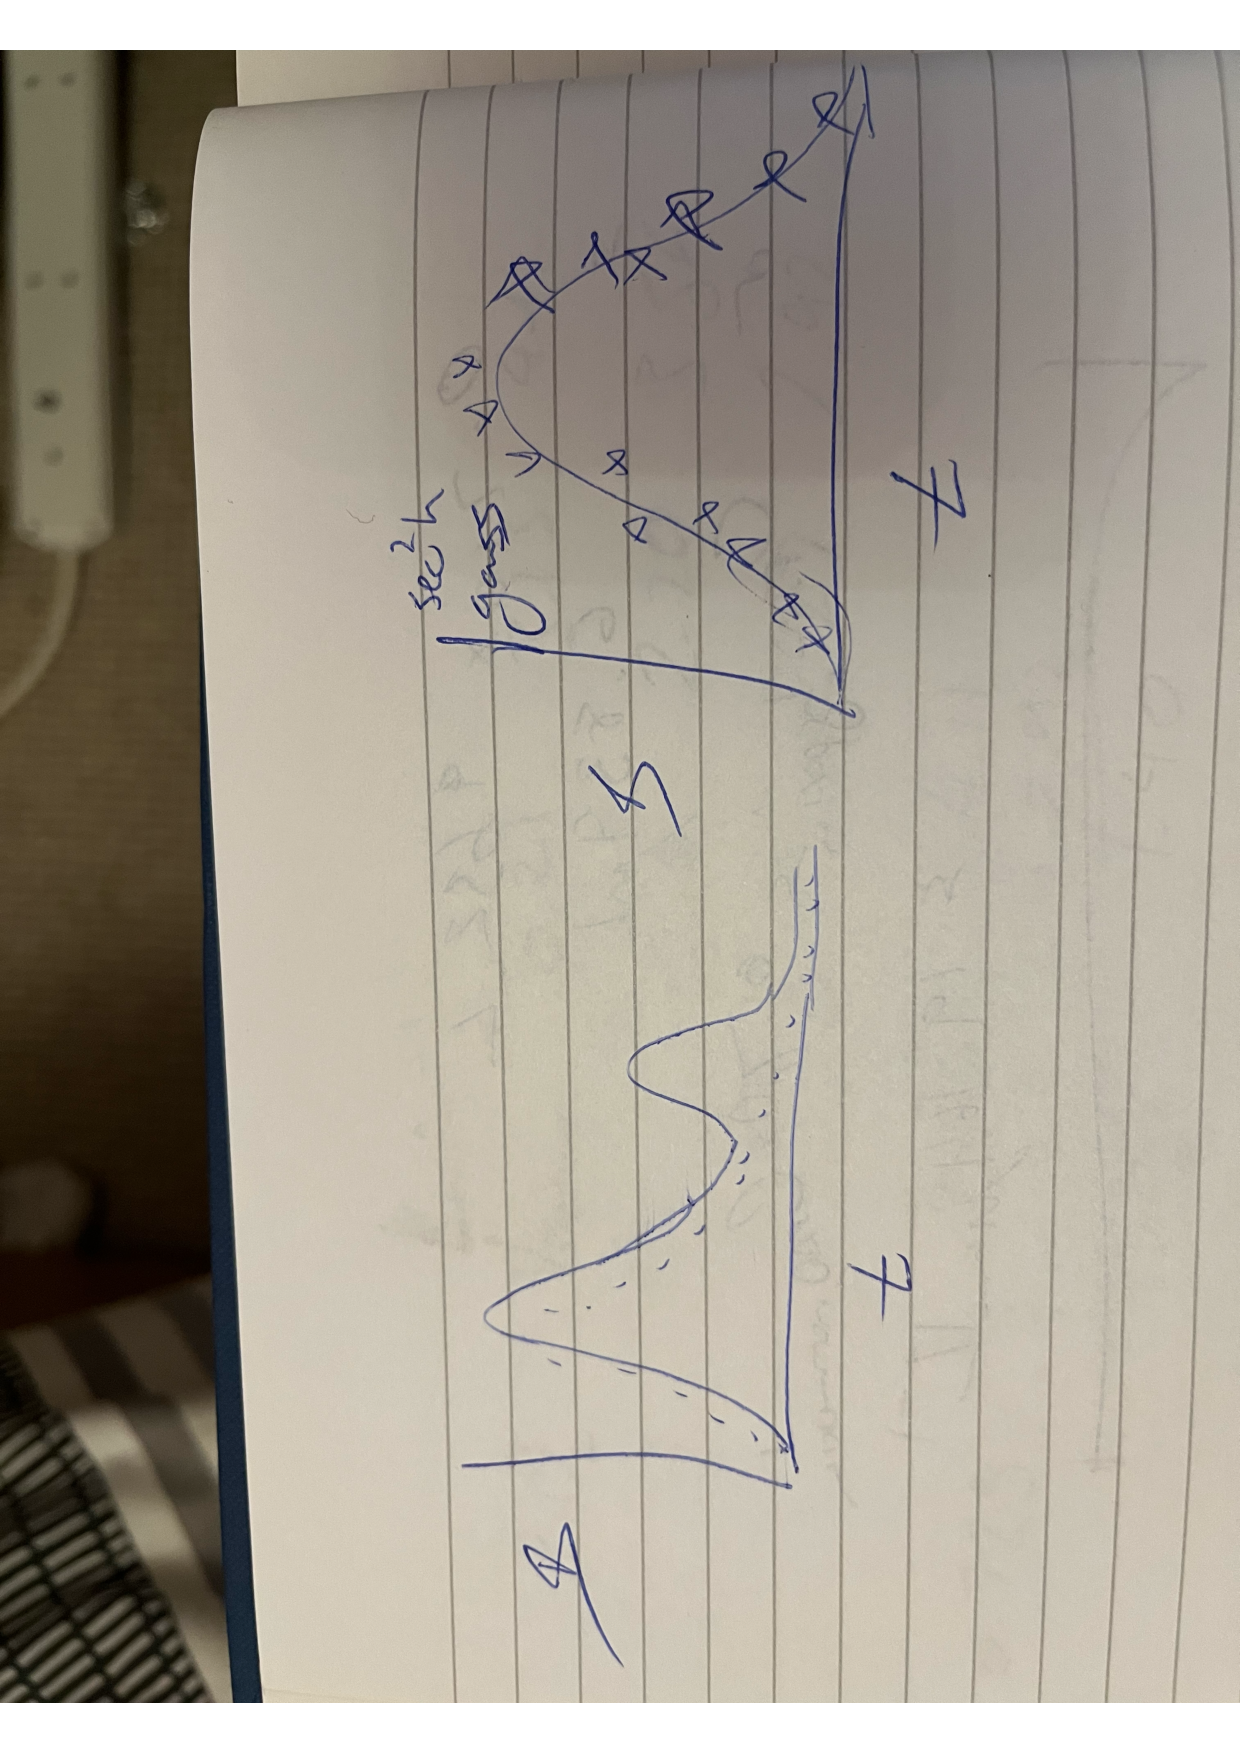
\includegraphics[angle = 270, width=0.5\linewidth]{figures/ratUCL/RoughDarkfieldFig.pdf}
    \caption{Caption}
    \label{fig:darkfieldGauss}
\end{figure}
If not accommodated in the unmixing process, this time-dependent dark current would result in poor convergence of minimising-function (\cref{eq:leastsquaretens}), $\varphi(\mathbf{x})$, to a solution $\mathbf{x}$, given that contamination in the SFLIM measurement, $\mathbf{M}$, is not accounted for in the model of endmember abundances, $\mathcal{A}$
\begin{equation}
    \varphi(\mathbf{x}) = \big\lvert\big\lvert \mathcal{A}\bullet_{3}\mathbf{x} - \mathbf{M}\big\rvert\big\rvert_{F}^{2}
\end{equation}
Ultimately this would yield unreliable and biased fluorophore concentrations. Instead, the affected time period could be masked out and this region is excluded when evaluating the minimising function. While the dark-current could be characterised by fitting a Gaussian or $\sec^{2}h$ for each pixel and then subtracted from the affected histogram but this could result in over-fitting in histograms with low photon counts - increasing sensitivity to noise. 
\begin{figure}
    \centering
    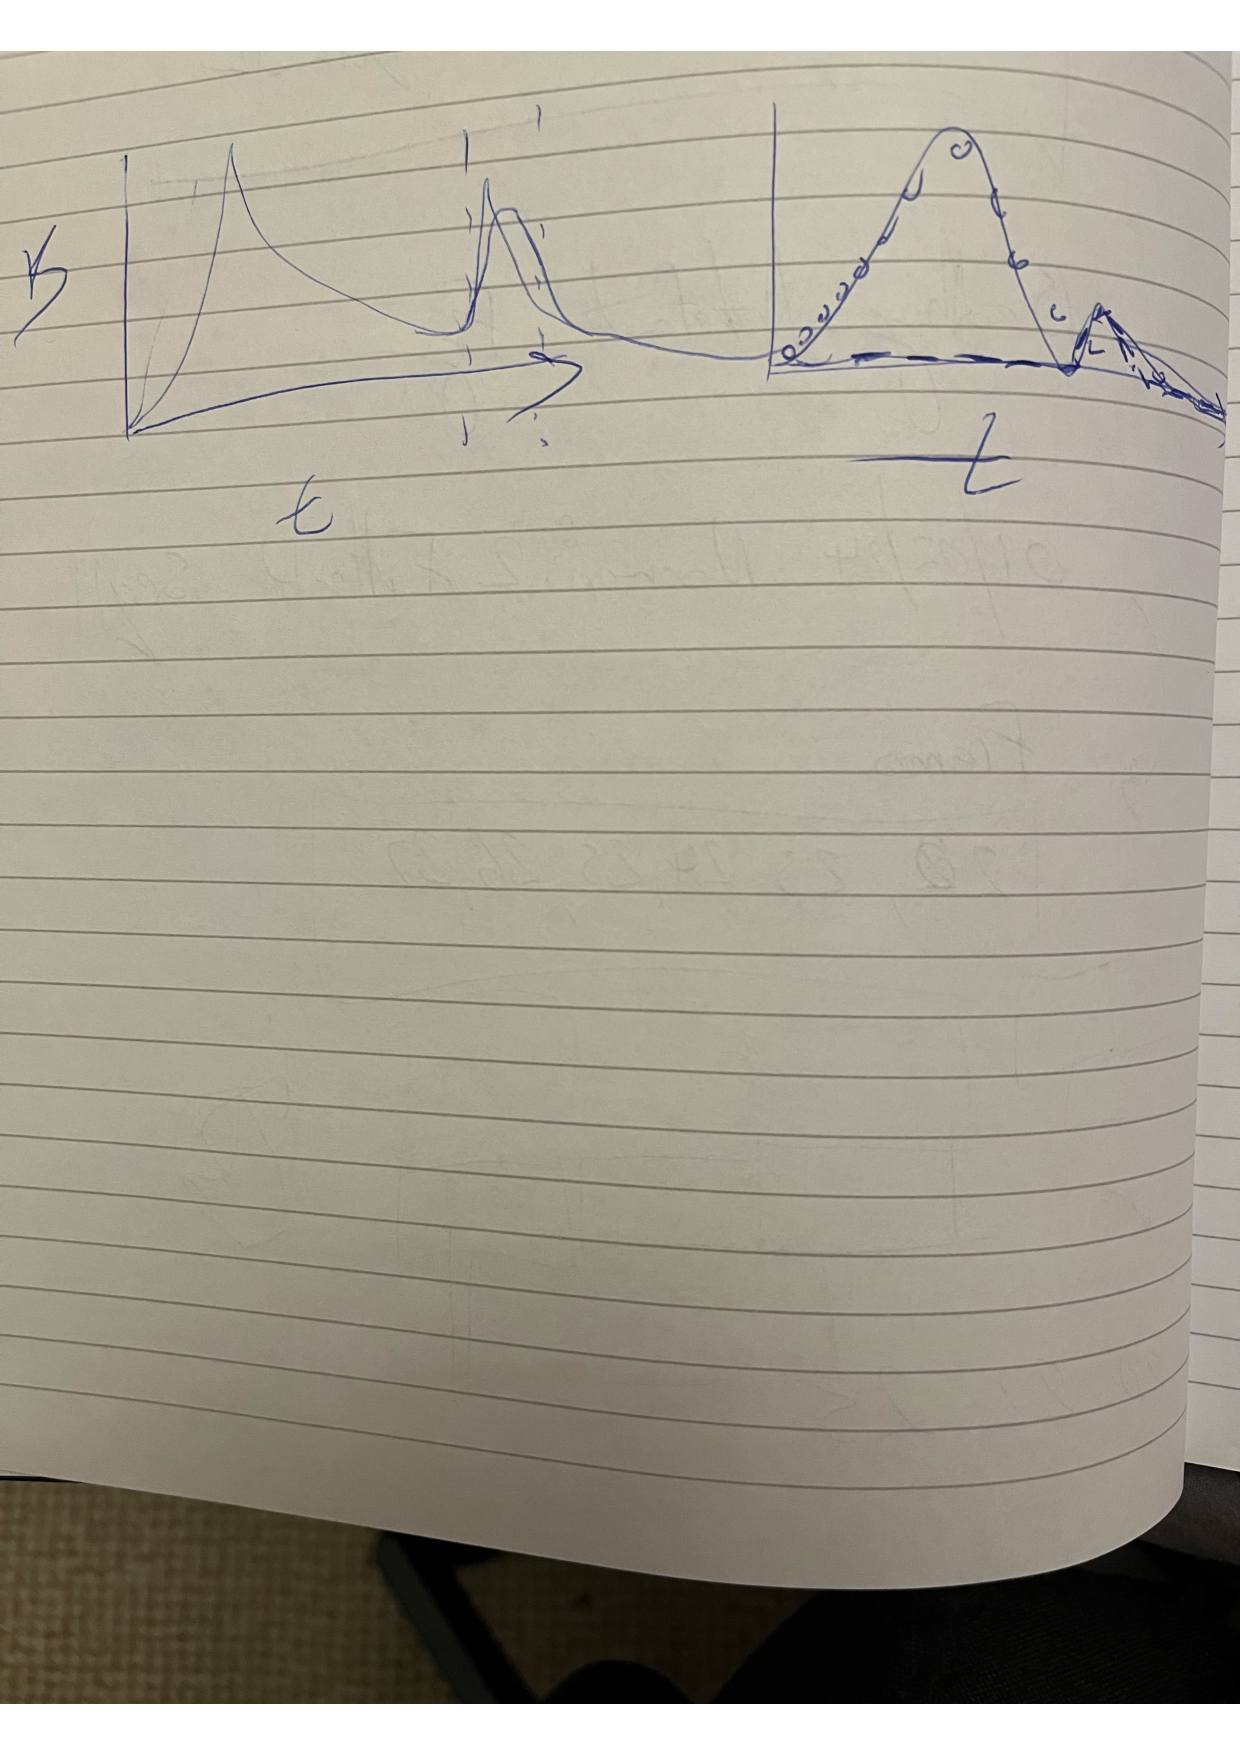
\includegraphics[width=0.5\linewidth]{figures/ratUCL/MaskedFittedFigure.pdf}
    \caption{Figure showing line plots with masked and fitted dark current.}
    \label{fig:maksed-fitteddarkcurrent}
\end{figure}
The masking approach however trades of leaving insufficient photons for unmixing when too many time bins are mask, and masking too few bins leaves the histogram still contaminated - biasing the recovered flourophore concentrations a masking window of XX pixels was selected to strike this balance which left on average YY photons used in the unmixing process after masking the dark-current and excluding the first $\approx \num{50}$ time-bins to remove the influence of the temporal response of the SFLIO device.
\\
As an aside, after removing these contaminated time-bins and summing the renaming photon counts to produce a fluorescence intensity image did not solve the problem of no resolvable details of the retina in the FLIMera images.
\begin{figure}
    \centering
    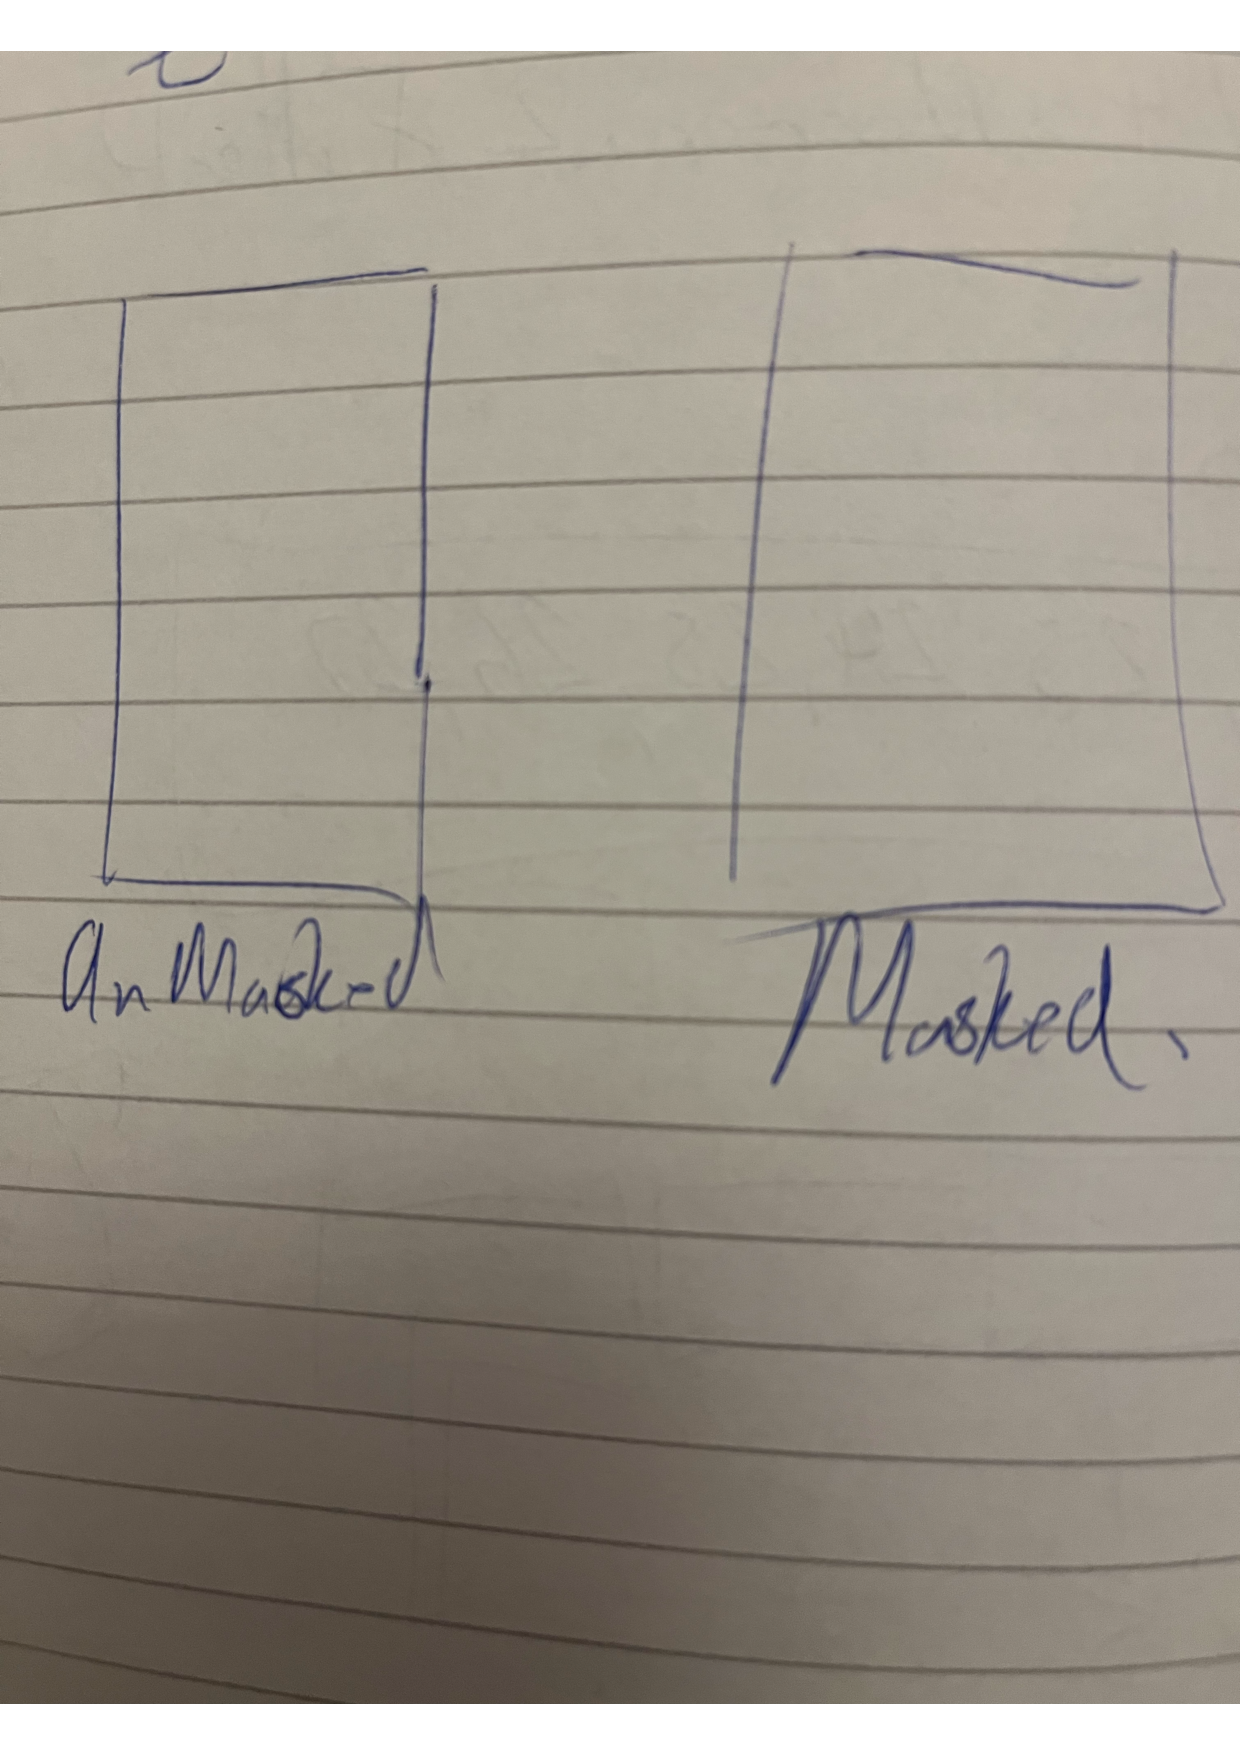
\includegraphics[width=0.5\linewidth]{figures/ratUCL/MaskedUnmaskedIntensityImage.pdf}
    \caption{Example SPAD fluorescence intensity image where the dark-current is masked and not masked. Images will look no different...}
    \label{fig:masked-unmaskedintensityimage}
\end{figure}
\FloatBarrier
\subsection{Trends in Retinal Fluorophore Concentration as a Response to Acute Hypoxia}\label{subsec:meanfluor}
The concentrations of the retinal fluorophores, FAD, AGE, and A2E, and can now be estimated from from SFLIM measurements with the SFLIM unmixing algorithm and any trends due to changes in oxygenation state can be established. Before this analysis, the SFLIM data is processed to mask malfunctioning pixels (\cref{sec:pixelmask}), the fluorescence decays are aligned in the time axis (\cref{sec:timealign}), and the time-bins affected by the previously mentioned dark-current are also masked.
The unmixing algorithm is performed on SFLIM measurements for each functional pixel on the SPAD array to produce images of relative fluorophore concentrations - shown in \cref{fig:rat1session1fluormaps,fig:rat2session2fluormaps,fig:rat1session3fluormaps}. 
\\
\begin{figure}
    \centering
    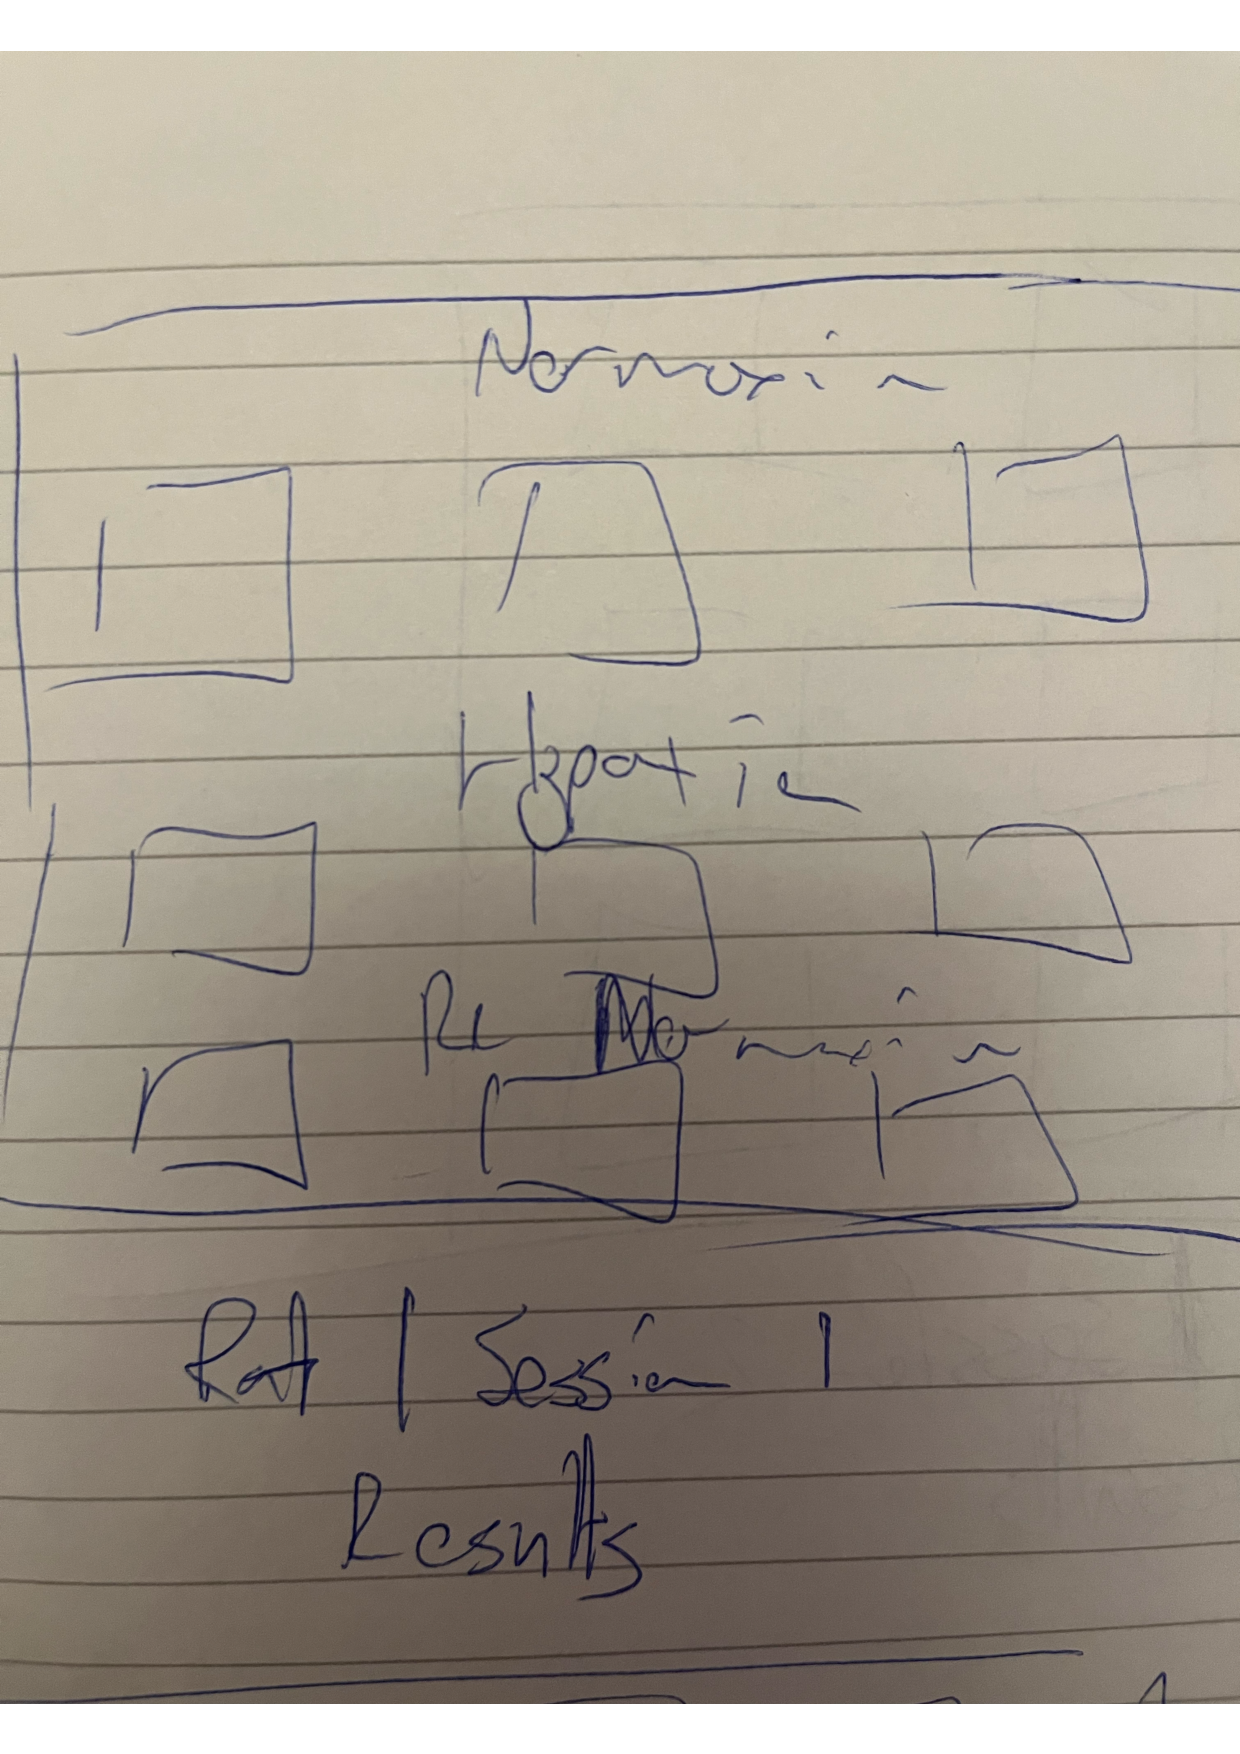
\includegraphics[width=0.5\linewidth]{figures/ratUCL/Rat1Session1FluorMapsRough.pdf}
    \caption{Caption}
    \label{fig:rat1session1fluormaps}
\end{figure}
\begin{figure}
    \centering
    
\includegraphics[width=0.5\linewidth]{figures/ratUCL/Rat2Session2FluorMaps.pdf}
    \caption{Caption}
    \label{fig:rat2session2fluormaps}
\end{figure}
\begin{figure}
    \centering
    
\includegraphics[width=0.5\linewidth]{figures/ratUCL/Rat1Session2FluorMaps.pdf}
    \caption{Caption}
    \label{fig:rat1session3fluormaps}
\end{figure}
Much like the integrated intensity maps in () these maps of fluorophore concentration show no variation across the image that could be correlated to structures in the retina. It would be expected that there would be a background level of FAD due to blood circulating around the choroid and areas of increased FAD around the arteries. 
Trends between the mean retinal fluorophore concentration and changes in oxygenation state can still be established using these unmixed fluorophore maps.
\subsubsection{Trends in Retinal Fluorophore Concentration Related to Changes in Oxygenation State}
For each rat, and each oxygenation state, the mean fluorophore concentration was calculated in terms of the number of photons of FAD, AGE, and A2E that were recovered. Now the prediction made at the start of this chapter - that FAD concentrations should decrease at acute hypoxia, relative to normoxic condition - can be evaluated. If this holds true, then it can be concluded that it is likely that retinal FAD has been detected.
In \cref{fig:rat1session1-trends, fig:rat2session2-trends, fig:rat1session3-trends} these mean concentrations are plotted and shows that in all three imaging sessions, the recovered FAD concentration decreased with acute hypoxia. 
\begin{figure}
    \centering
    \includegraphics[width=0.5\linewidth]{figures/ratUCL/FADTrends.png}
    \caption{\textcolor{red}{place holder graphic}}
    \label{fig:rat1session1-trends}
\end{figure}
\begin{figure}
    \centering
    \includegraphics[width=0.5\linewidth]{figures/ratUCL/AGETrends.png}
    \caption{Caption}
    \label{fig:rat2session2-trends}
\end{figure}
\begin{figure}
    \centering
    \includegraphics[width=0.5\linewidth]{figures/ratUCL/A2ETrends.png}
    \caption{Caption}
    \label{fig:rat1session3-trends}
\end{figure}
This assertion should not be without scrutiny. Error bars were calculated as the standard error of the mean of repeated measurements of mean retina fluorophore concentrations, constructed from splitting the SFLIM measurements into 10 short sub-acquisitions and recovering retinal fluorophores. As can be seen, most of the reduction in FAD between normoxia and hpyoxia can be attributed to variance in the measurements due to low-photon counts and the possibility of the fluorophores becoming bleached. 
Additionally, it was predicted that when the rat transitions back to normoxia from hypoxia the FAD concentration should return to its previous levels. This is not seen in the the recovered mean concentrations of FAD. In the one instance where the rat was sacrificed and a SFLIM dataset was acquired the FAD concentration does not decay to zero when all metabolic processes cease. A paired student T-test was then carried out on each pair of change in oxygenation to assess whether the trends in retinal fluorophores is due to a change in the oxygenation of the rat or simple variation in the measurements due to high noise.


\FloatBarrier
\subsection{Assessing Statistical Significance of FAD Response}\label{subsec:ttest}
The error, or variation, in the recovered fluorophore concentrations is on the same order as the change in mean-concentration between oxygenation states. This introduces uncertainty in whether the change in FAD concentration that was measured is actually caused by varying the consumption of oxygenation in the rat or simply variation in the measurement. To address this concern a ``Student Paired t-test'' can be performed on the recovered fluorophore concentration to bound the probability, $p$, of the change we measured being due to variation in the measurement - termed "null hypothesis" - with the probability that the induction of hypoxia did cause a change in the FAD concentration with probability $1-p$. 
To perform a Student Paired t-test. The standard error of the mean of differences between the recovered concentrations for two oxygenations states, $x_{i}$ and $y_{i}$ is calculated to derive the T-statistic, $T = \nicefrac{\Bar{\Delta}_{xy}}{\Bar{\sigma}_{xy}}$. Where $\Bar{\Delta}_{xy}$ is the mean difference between two oxygenation states, $x$ and $y$, 
\begin{equation}
    \Bar{\Delta}_{xy} = \overline{ x_{i} - y_{i}}
\end{equation}
and $\Bar{\sigma}_{xy}$ is the standard error computed from the standard deviation, $\sigma_{xy}$, over $n$ samples.
\begin{equation}
    \Bar{\sigma}_{xy} = \frac{\sigma_{xy}}{\sqrt{n}}
\end{equation}

By comparing the T-statistic with a $t$-distribution (\cref{eq:tdist}) with $n$ degrees-of-freedom, the $p$-value can be extracted to give a probability of the null-hypothesis. 
\begin{equation}\label{eq:tdist}
    f(t) = \frac{\Gamma(\frac{n+1}{2})}{\sqrt{\pi}\Gamma(\frac{n}{2})}\Bigg(1 + \frac{t^{2}}{n}\Bigg)^{-(\frac{n+1}{2})}
\end{equation}For each fluorophore the change in concentration is calculated as the percentage change of total number of photons recorded over two different oxygenation states. The $p$-value is then computed using a $t$-distribution look-up table (``\textit{scipy}'' \textit{python} package) and is shown in \cref{tab:ttestMain}. 

\begin{table}
    \begin{subtable}[t]{0.9\textwidth}
    \centering
    \sisetup{table-alignment-mode=format, round-mode=figures, table-column-width=1.5cm}
    \small
    \begin{tabular}{|p{3.2cm}|  S[round-precision=4]|
                                S[round-precision=2]|
                                S[round-precision=4]|
                                S[round-precision=2]|
                                S[round-precision=4]|
                                S[round-precision=2]|
                                S[round-precision=4]|
                                S[round-precision=2]|
                                S[round-precision=4]|
                                S[round-precision=2]|}
        \hline
        & \multicolumn{2}{c|}{Rat 1 - Session 1} & \multicolumn{2}{c|}{Rat 2 - Session 1} & \multicolumn{2}{c|}{Rat 1 - Session 2} \\
        \hline
       Change in Oxy.& {$\Delta_{FAD}$} & {$p$-value}  & {$\Delta_{FAD}$} & {$p$-value}  & {$\Delta_{FAD}$} & {$p$-value} \\
        State & {(\%)} & & {(\%)} & & {(\%)} &\\
       \hline
       Norm. To Hyp. & \num{-31.306511215525244} & \num{4.78989243667469e-07} & \num{-54.83078399530178} & \num{5.535602434791192e-09} & \num{-32.76058614849388} &\num{5.438630613110299e-09}\\
       \hline
       Hyp. To Nor. 2 & \num{7.896276165081215} & \num{0.04001956386363361} & 14.76457257722695 & \num{4.7271147283432893e-07} & \num{51.55500731722816}& \num{2.053319524750847e-06}\\
       \hline
       Norm. To Norm. 2 &  \num{-24.501622691262938} & \num{8.510036758754948e-09} & \num{-43.60961563462101} & \num{2.926951097621746e-08} & \num{22.68463380231996} &\num{2.520271452591082e-04}\\
       \hline
       Norm. To Death & &  &\num{-43.609523917005596}& \num{2.9270614725268114e-08}& &  \\
       \hline
       Hyp. To Death &  &  &\num{14.764680152018073}& \num{4.726990805630476e-07}&  &  \\
       \hline
       Norm. 2 To Death & & & {\num[round-mode=places, round-precision=4]{0.00011}} &\num{0.05743584614696069}& & \\
       \hline
                                
    \end{tabular}
    \caption{sub table FAD}
    \label{tab:ttestFAD}
    \end{subtable}
    
    \begin{subtable}[t]{0.9\textwidth}
    \centering
    \sisetup{table-alignment-mode=format, round-mode=figures, table-column-width=1.5cm}
    \small
    \begin{tabular}{|p{3.2cm}|  S[round-precision=4]|
                                S[round-precision=2]|
                                S[round-precision=4]|
                                S[round-precision=2]|
                                S[round-precision=4]|
                                S[round-precision=2]|
                                S[round-precision=4]|
                                S[round-precision=2]|
                                S[round-precision=4]|
                                S[round-precision=2]|}

        \hline
        & \multicolumn{2}{c|}{Rat 1 - Session 1} & \multicolumn{2}{c|}{Rat 2 - Session 1} & \multicolumn{2}{c|}{Rat 1 - Session 2} \\
        \hline
       Change in Oxy.& {$\Delta_{AGE}$} & {$p$-value}  & {$\Delta_{AGE}$} & {$p$-value}  & {$\Delta_{AGE}$} & {$p$-value} \\
        State & {(\%)} & & {(\%)} & & {(\%)} &\\
       \hline
       Norm. To Hyp. & \num{36.73845540879449} & \num{1.2129855908953851e-09} & \num{55.94262439767155} & \num{0.1588847726902607} & \num{-4.869533327623472} &\num{0.01476854947998337}\\
       \hline
       Hyp. To Nor. 2 & \num{-36.47776055506893} & \num{5.458684853053609e-10} & \num{-67.14473694997025} & \num{0.028701101342988936} & \num{-4.58604064439413}& \num{0.03315636788775767}\\
       \hline
       Norm. To Norm. 2 &  \num{0.5207084290772277} & \num{0.378107436641914} & \num{-15.264845593890513} & \num{0.04101290831611819} & \num{-9.376587991622035} &\num{0.004406940283828267}\\
       \hline
       Norm. To Death & &  &\num{-15.264100742018567}& \num{0.005133755889685807}& &  \\
       \hline
       Hyp. To Death &  &  &\num{-67.14432734548367}& \num{3.682486022535063e-08} &  &  \\
       \hline
       Norm. 2 To Death & & & {\num[round-mode=places, round-precision=4]{0.000819894114190679}} &\num{0.032766934545733456}& & \\
       \hline                                
    \end{tabular}   
    \caption{sub table AGE}
    \label{tab:ttsetAGE}
    \end{subtable}

    
    \begin{subtable}[t]{0.9\textwidth}
    \centering
    \small
    \sisetup{table-alignment-mode=format, round-mode=figures, table-column-width=1.5cm}
    \begin{tabular}{|p{3.2cm}|  S[round-precision=4]|
                                S[round-precision=2]|
                                S[round-precision=4]|
                                S[round-precision=2]|
                                S[round-precision=4]|
                                S[round-precision=2]|
                                S[round-precision=4]|
                                S[round-precision=2]|
                                S[round-precision=4]|
                                S[round-precision=2]|}   
        \hline
        & \multicolumn{2}{c|}{Rat 1 - Session 1} & \multicolumn{2}{c|}{Rat 2 - Session 1} & \multicolumn{2}{c|}{Rat 1 - Session 2} \\
        \hline
       Change in Oxy.& {$\Delta_{A2E}$} & {$p$-value}  & {$\Delta_{A2E}$} & {$p$-value}  & {$\Delta_{A2E}$} & {$p$-value} \\
        State & {(\%)} & & {(\%)} & & {(\%)} &\\
       \hline
       Norm. To Hyp. & \num{62.13010322707054} & \num{1.0740993673380998e-11} & \num{5.027149310079019} & \num{0.08183947292419991} & \num{-26.69017034022325} &\num{5.154642206973885e-09}\\
       \hline
       Hyp. To Nor. 2 & \num{-42.71268278804473} & \num{1.830243802194944e-12} & \num{-28.48335445402891} & \num{0.05633120789198803} & \num{6.639735558159754}& \num{3.0127109988835988e-06}\\
       \hline
       Norm. To Norm. 2 &  \num{26.420008804075852} & \num{2.0075775208559094e-07} & \num{-23.65399336336594} & \num{0.07484643982404204} & \num{-20.46661779529254} &\num{3.5187463156723894e-08}\\
       \hline
       Norm. To Death & &  &\num{-23.654034685580303}& \num{5.615975463161401e-05} & &  \\
       \hline
       Hyp. To Death &  &  &\num{-28.483398694681544}& \num{1.3725568075817538e-07} &  &  \\
       \hline
       Norm. 2 To Death & & &{\num[round-mode=places, round-precision=5]{-0.00005589514560848622}} & \num{0.37480529225054726} & & \\
       \hline
    \end{tabular}
    \caption{sub table A2E}
    \label{tab:ttestA2E}
\end{subtable}
\caption{The $p$-value for the measured changes in the concentration of the fluorophores FAD, AGE, and A2E has been calculated for each pair of oxygenation states for each imaging session: Normoxia to Hypoxia; Hypoxia back to Normoxia; between the both measurements of a Normoxic state; and permutations where the rat was sacrificed. Lower $p$-values indicate a higher likelihood that a physiological change was detected in the SFLIM measurements - variation in the results is not simply due to sample variation}
\label{tab:ttestMain}
\end{table}
For FAD over all 3 imaging sessions a similar decrease in apparent FAD concentration is recorded with $p$-values indicating a high confidence that ``something'' has changed in response to changing the rats physiology. This is follows the expectations set out in the beginning of the chapter but there are some disagreements. Interestingly, what is not seen is the concentration of FAD returning to its initial value after the rat is returned to a normoxic state after being in hypoxia - implying that the FAD is not being restored when after no longer being hypoxic. A disagreement in the recovered FAD concentrations with the expected change due to physiology is also seen in SFLIM measurements from where the rat is sacrificed - all metabolic functions have ceased - and all the FAD in the retina should have dissipated. While the measured concentration of FAD does show a decrease from the initial normoxic state to death (albeit not to zero) the \textit{post-mortem} FAD concentration is the same or higher when the rat is hypoxic, or the same when compared to when the rat is normoxic after having been hypoxic. This true for all 3 fluorophores when comparing this second normoxic state to \textit{post-mortem} fluorophore concentrations.
This incongruence between the recovered fluorophore concentrations and what was expected from the variations of physiology required further analysis into whether the SFLIM measurements actually show variation between oxygenation states. In the next section, a simple technique of Principle Components Analysis is used on the spectral domain to uncover changes between oxygenation states to motivate the hypothesis that changes in recovered FAD changes are correlated to changes in SFLIM measurements.


\FloatBarrier
\subsection{Comparing Detected Changes with PCA and Spectral Angle Maps}\label{subsec:pcarat}
To reinforce the connection between the recovered FAD concentration and oxygenation state, the technique Principle Components Analysis (PCA) can be used to affirm two hypotheses: that the SFLIM measurements show changes in the spectra and lifetime domain as a response to changing physiology in the rat; and SFLIM unmixing algorithm is capable of uncovering these changes with accuracy and precision sufficient to detect FAD. PCA uses a coordinate transformation to reduce the number of orthonormal bases (dimensions) in a dataset to those which exhibit the most variation or information. This technique is particularly useful for distilling higher-dimensional datasets into typically 2 dimensions that can be visualised by humans and is readily used for identifying unique endmembers in spectral images \addcite. The SFLIM measurements of in-vivo rat retinas can be reduced into spectral images and analysed using PCA to identify the fluorescence emission spectra is changing as a response to hypoxia - with premise being that each oxygenation state will occupy unique regions in the plane of 2 principal components.
\subsubsection{PCA Maps of SFLIM Data}
Before the principal components can be used, the SFLIM measurements are formed into spectral images by summing across the time access of the $I(x,y,t,\lambda)$ volume and area normalised to form $I'(x,y,t,\lambda)$.
\begin{equation}
    I'(x,y,t,\lambda) = \frac{I(x,y,t,\lambda)}{\int_{0}^{\infty}I(x,y,t,\lambda)d\lambda}
\end{equation}
The area normalisation allows for spectra of the same pixel on the SPAD $(XY)$ but differing oxygenation state to be compared. The 4D point-clouds - 1 dimension for each spectral band - for each oxygenation states are then concatenated together such that the principal components are optimised for the every oxygenation state. The first two principle components are then found and the corresponding coordinate transformation is applied to produce 2D point-clouds which are colour-coded for each oxygenation state in \cref{fig:ratPCA}.
%\printinunitsof{in}\prntlen{\textwidth}

\begin{figure}
    \centering
    \begin{annotatedFigure}{\includegraphics[width=0.9\textwidth]{figures/ratUCL/RatOxygenationPCAPlot.pdf}}
        \annotatedFigureText{0.01,0.97}{black}{0.3}{a)}
        \annotatedFigureText{0.53,0.97}{black}{0.3}{b)}
        \annotatedFigureText{0.24,0.50}{black}{0.3}{c)}

    \end{annotatedFigure}
    \caption{First 2 principal components of spectra images recorded of the pair of rats that were imaged over 3 sessions (a-c). The normoxic and hypoxic point clouds occupying separate regions in (a) and (c) indicates that as a response to hypoxia the fluorescence emission of the retina does change. The fact that the other oxygenation states do not form unique clusters does indicate either the restoration of metabolic function after hypoxia takes place over longer than expected time scales and/or a shortcoming in the SFLIM unmixing algorithm and SFLIO device.}
    \label{fig:ratPCA}
\end{figure}
In \cref{fig:ratPCA}a and \cref{fig:ratPCA}c, there is visibly separate regions occupied by the spectra of the normoxic and hypoxic states indicating that there is a change in the fluorescence emission spectra in the rat retina as a response to acute hypoxia. However, what is not evident in \cref{fig:ratPCA}a-c - but was expected - would be significant overlap between the regions of the initial normoxic state and the spectra recorded after the rat was brought back to normoxia after being hypoxic. Instead it appears that the measurements of the second period of normoxia highly overlap the hypoxic measurements which could be explained as a combination of both physiological factors and a limitation of the SFLIO device and SFLIM unmixing algorithm. When transitioning between oxygenation states the rats were allowed a period of \qtyrange{2}{3}{\minute} to allow metabolic functions to stabilise or return to normal. It is likely that if this refractory period was not long enough then this would result in the metabolites such as FAD, and AGE not being fully replenished and being produced at a healthy rate before the next SFLIM dataset was recorded. As to the high overlap between every oxygenation state when the first rat was re-imaged, phototoxic damage to the retina from the long and intense exposure of the previous imaging session could have disrupted the production of metabolites, FAD and AGE, and damaged the RPE which is responsible for the fluorescence from A2E \addcite. The lasers exposure would be estimated to be around \numproduct{2.5 x 3} as intense (power per unit area~\cite{yao2021understanding}) as the safety threshold for safe human imaging and sustained for over \qty{30}{\minute} and could readily result in permanent damage to the rats retina.
\FloatBarrier
\subsubsection{Quantitative Assessment of }
The perceived separation in the map of principal components in \cref{fig:ratPCA} can be quantified using the metric of the Spectral Angle Map (SAM), shown in \cref{eq:sam2} to calculate the overlap between pairs of oxygenation states $\mathbf{a}$ and $\mathbf{b}$.
\begin{equation}\label{eq:sam2}
    \varphi = \frac{\mathbf{a}\cdot \mathbf{b}}{\lvert \mathbf{a} \rvert\,\lvert \mathbf{b} \rvert}
\end{equation}
For every combination of 2 oxygenation states the spectral angle, $\varphi$, is computed pointwise, allowing for the mean overlap to be calculated. 


To Do Make a table of spectral angles - do it in the style of the p-value one but a seperate table for each rat.
Write about results of this - then sections done!
\FloatBarrier
\section{Conclusions}\label{sec:uclconcs}
\section{Future Work and Experimental Improvements}

\section{Outline / TO DO}
\begin{itemize}
        \item Assessing Results using spectral angle maps and PCA
        \begin{itemize}
            \item To assess whether the SFLIM unmixing algorithm was detecting a change rather than simply variations due to photo bleaching, changes in blood oxygenation spectral angles were calculated for each point in the image.
            \item The sflim data for each rat was then concatenated forming a 4D point cloud of spectra and PCA was applied to reduce the dimensionality to 2. 
            \item It was observed that normoxia and hypoxia formed unique clusters with separation X. When transiting back to normoxia from hypoxia and then onto death there was no change in the clustering
            \item it would have been expected for the two normoxia data sets to exhibit high overlap and the hpyoxic and post mortem data would form unique clusters
        \end{itemize}
        \item Future Work and the benefit of hindsight
        \begin{itemize}
            \item A more rigourous model of the fluorescence in the retina would enable the effect of absorption due to retinal vasculature and lens fluorescence to be understood.
            \item to eliminate the possibility the visotears was responsible for the lack of spatial variation in the images a SFLIM measurement of it should be recorded. This could be applied to the existing SFLIM data of the rats by including it as an additional endmember. The current spectral bands would not be optimised for this but it would nonetheless serve to eliminate it as a candidate.
            \item Further in-vitro experiments should have been performed to better understand the sensitivity of the unmixing approach in experimental setting. This would take the form capillary tubes implanted in the retinal plane of an artificial eye and filled with varying concentrations and mixtures of FAD and other fluorophores.
        \end{itemize}
\end{itemize}

\begin{itemize}
    \item While a high quality image could be formed on the sCMOs camera which clearly shows the vascular structure of the retina could be formed - albeit polluted by glare in the centre of the vision. A sufficient image could not be formed on the FLIMera but there is sufficient signal to attempt SFLIM unmixing. This could be due to the low fluorescence contrast as evidenced by the fluorescence intensity image recorded with a lp500 filter in the SCMOs camera. 
    \item Can't map FAD across the retina but can use the signal to extract a general trend in the FAD concentration wrt oxygenation.
    \item In the histograms recorded by the FLIMera there was also the addition Gaussian like thermal noise characteristic that was ultimately corrected by simply neglecting these values in the calculation of the cost function of the minimisation process (phi). While this does decrease the overall energy in the signal what is left should be capable of capturing both the long and short lifetime dynamics.
    \item A brief comparison of the possible dark field correction methods yielded no significant change in the recovered concentration of retinal FAD  - dark-field correction by fitting a modified Gaussian to the artefact and subtracting from each histogram, masking the effected time bins, and simple fitting through the artefact.
\end{itemize}


